% =============================================
% File: chapters/methodology.tex
% Chương 3: Phương pháp thực hiện
% =============================================

\chapter{PHƯƠNG PHÁP THỰC HIỆN}
\label{chap:phuongphap}

Chương này trình bày toàn bộ quy trình và phương pháp cụ thể được áp dụng
trong đề tài, gồm hai hướng song song: (1)~\textbf{hướng điều khiển cổ điển}
— thu thập dữ liệu, nhận dạng hàm truyền động cơ, tối ưu tham số bộ điều
khiển tầng bằng giải thuật di truyền, xây dựng mạng ANN dự đoán tham số
thích nghi, và triển khai trên vi điều khiển ESP32; (2)~\textbf{hướng học
tăng cường} — xây dựng môi trường mô phỏng trong Isaac Lab, huấn luyện
chính sách điều khiển bằng thuật toán PPO và xuất trọng số để triển khai
thực tế.


% ==============================================
\section{Quy trình nghiên cứu tổng quan}
% ==============================================

Nghiên cứu được thực hiện theo hai hướng song song với 6 giai đoạn chính:

\begin{enumerate}
    \item \textbf{Giai đoạn 1 — Thu thập dữ liệu thực nghiệm:}
    Vận hành động cơ NF5475 theo giao thức kích thích bậc thang ở 5 mức PWM,
    đọc phản hồi vận tốc qua encoder 200~PPR và ghi log về máy tính qua
    cổng Serial (115\,200~baud).

    \item \textbf{Giai đoạn 2 — Nhận dạng hàm truyền:}
    Sử dụng MATLAB System Identification Toolbox (\texttt{tfest}) để xác định
    hàm truyền $G_{\text{vel}}(s)$ của động cơ; rời rạc hóa bằng phương pháp
    Tustin để phục vụ tối ưu GA.

    \item \textbf{Giai đoạn 3 — Tối ưu bộ điều khiển bằng GA:}
    Áp dụng giải thuật di truyền trên mô hình rời rạc để tìm bộ tham số tối
    ưu $(K_{pp}^*, K_{ip}^*, K_{dp}^*, K_{pv}^*, K_{iv}^*)$ cho bộ điều
    khiển cascade PID-vị trí + PI-vận tốc, tại nhiều mức setpoint.

    \item \textbf{Giai đoạn 4 — Xây dựng và huấn luyện ANN:}
    Từ bộ tham số GA tối ưu tại 9 setpoint vận tốc (250--2250~RPM),
    huấn luyện mạng ANN có khả năng dự đoán tham số PI thích nghi theo
    setpoint và sai số vận tốc hiện tại.

    \item \textbf{Giai đoạn 5 — Triển khai trên ESP32:}
    Cài đặt vòng điều khiển PI với tham số do ANN dự đoán lên vi điều khiển
    ESP32, thực nghiệm vận tốc và đánh giá đáp ứng hệ thống.

    \item \textbf{Giai đoạn 6 — Huấn luyện RL trong Isaac Lab:}
    Song song với hướng điều khiển cổ điển, xây dựng môi trường mô phỏng
    vật lý trong Isaac Lab và huấn luyện chính sách điều khiển chuyển động
    toàn thân bằng thuật toán PPO với curriculum 3 pha dựa trên hiệu suất.
    Sau huấn luyện, trọng số mạng Actor được xuất sang ONNX để triển khai
    thực tế.
\end{enumerate}

% ==============================================
\section{Mô tả hệ thống robot hai chân}
% ==============================================

\subsection{Kiến trúc tổng thể}

Robot Legged V3 là robot hai chân có bánh xe (\textit{wheeled bipedal robot}),
trong đó mỗi chân được dẫn động bởi cơ cấu song song 5-bar. Bánh xe được gắn
tại điểm cuối chân (end-effector), cho phép robot vừa di chuyển bằng bánh vừa
thay đổi chiều cao thân thông qua điều khiển góc khớp.

\begin{figure}[H]
    \centering
    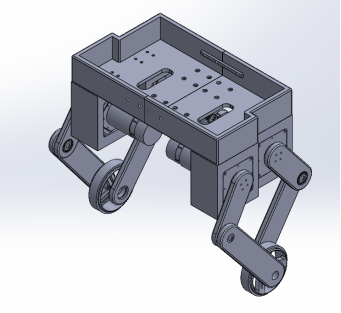
\includegraphics[width=0.45\textwidth]{figure/mohinhtongthe.png}
    \caption{Mô hình tổng thể robot Legged V3}
    \label{fig:robot_overview}
\end{figure}

Robot gồm thân chính phía trên, hai cụm chân đối xứng qua mặt phẳng giữa và
bánh xe đặt tại điểm cuối mỗi chân. Mỗi cụm chân sử dụng hai động cơ NF5475
có encoder để điều khiển hai thanh chủ động; hai thanh bị động tạo thành chuỗi
động học kín, xác định vị trí điểm cuối $P$ để đặt trục bánh xe.

\begin{figure}[H]
    \centering
    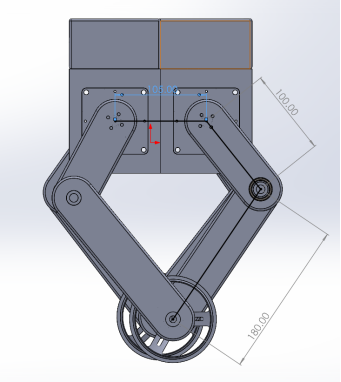
\includegraphics[width=0.45\textwidth]{figure/robotmohinh.png}
    \caption{Mô hình 3D robot Legged V3}
    \label{fig:robot_3d}
\end{figure}

Hệ thống được chia thành ba cấp:
\begin{itemize}
    \item \textbf{Cấp cơ khí:} Khung nhôm định hình, hai cơ cấu 5-bar
    parallel, trục bánh xe.
    \item \textbf{Cấp dẫn động:} Bốn động cơ DC NF5475 (hai mỗi chân)
    kết hợp encoder quang học 200 PPR.
    \item \textbf{Cấp điều khiển:} Vi điều khiển ESP32 WROOM-32, mạch
    driver L298N, giao tiếp Serial/UART với máy tính.
\end{itemize}


\subsection{Cơ cấu 5-bar parallel}

Ký hiệu các thành phần cơ cấu được quy ước trong Bảng~\ref{tab:5bar_notation}.

\begin{table}[H]
    \centering
    \caption{Ký hiệu các thành phần cơ cấu 5-bar parallel}
    \label{tab:5bar_notation}
    \renewcommand{\arraystretch}{1.3}
    \begin{tabular}{|c|l|p{7cm}|}
    \hline
    \textbf{Ký hiệu} & \textbf{Tên} & \textbf{Mô tả} \\
    \hline
    $A_1,\,A_2$ & Khớp chủ động & Hai khớp quay cố định trên thân,
                  truyền động bởi động cơ NF5475 \\
    \hline
    $B_1,\,B_2$ & Khớp bị động & Nối giữa thanh chủ động và thanh bị động \\
    \hline
    $P$         & Điểm cuối     & Vị trí gắn cụm bánh xe \\
    \hline
    $d$         & Khoảng cách gốc & Khoảng cách $A_1A_2$ \\
    \hline
    $L_{act}$   & Thanh chủ động & Chiều dài $A_1B_1$ và $A_2B_2$ \\
    \hline
    $L_{pas}$   & Thanh bị động  & Chiều dài $B_1P$ và $B_2P$ \\
    \hline
    \end{tabular}
\end{table}

Thông số hình học của cơ cấu trong đề tài:

\begin{table}[H]
    \centering
    \caption{Thông số hình học cơ cấu 5-bar parallel}
    \label{tab:5bar_params}
    \renewcommand{\arraystretch}{1.3}
    \begin{tabular}{|l|c|c|}
    \hline
    \textbf{Thông số} & \textbf{Ký hiệu} & \textbf{Giá trị} \\
    \hline
    Khoảng cách hai khớp chủ động & $d = A_1A_2$ & 105 mm \\
    Chiều dài thanh chủ động      & $L_{act}$    & 100 mm \\
    Chiều dài thanh bị động       & $L_{pas}$    & 180 mm \\
    \hline
    \end{tabular}
\end{table}

Ưu điểm so với chân nối tiếp: (i)~độ cứng vững cao hơn do tải phân phối
trên hai thanh bị động, (ii)~khối lượng phần chuyển động nhỏ vì động cơ
đặt tại gốc cố định, (iii)~giảm số bậc tự do cần điều khiển xuống còn 2.


% ==============================================
\section{Thu thập dữ liệu và nhận dạng hàm truyền}
\label{sec:data_sysid}
% ==============================================

\subsection{Quy trình thu thập dữ liệu}

Dữ liệu đặc tính động cơ DC NF5475 được thu thập theo giao thức kích thích
bậc thang (\textit{step-input protocol}). Vi điều khiển ESP32 lần lượt áp
5 mức PWM cố định: $20\%$, $40\%$, $60\%$, $80\%$, $100\%$ (tương ứng 51,
102, 153, 204, 255 đơn vị 8-bit), mỗi mức duy trì trong \textbf{10 giây}.

Vận tốc tức thời được tính sau mỗi chu kỳ lấy mẫu $T_s = 0{,}01\;\text{s}$:
\begin{equation}
    v(k) = \frac{n_{\text{xung}}(k)}{200} \cdot \frac{60}{T_s}
    \qquad [\text{RPM}]
    \label{eq:vel_calc}
\end{equation}
trong đó $n_{\text{xung}}(k)$ là số xung encoder (200~PPR) tích lũy trong
khoảng $[kT_s,\,(k{+}1)T_s)$. Bộ ba $(t,\;v(k),\;u(k))$ được truyền qua
cổng Serial (115\,200~baud) và ghi thành file CSV trên máy tính, thu được 5
file CSV ứng với 5 mức kích thích, tổng khoảng 5\,000 mẫu dữ liệu thô.

\subsection{Tiền xử lý dữ liệu}

\textbf{Chọn file nhận dạng.}
Trong số 5 file thu được, file có mức PWM 80\%
(\texttt{motor\_data\_004.csv}) được chọn làm dữ liệu nhận dạng vì đảm bảo
tỉ số tín hiệu trên nhiễu cao, chưa xảy ra bão hòa tốc độ, và đại diện tốt
cho vùng hoạt động tuyến tính của động cơ.

\textbf{Thêm đoạn trước zero (zero-prepend).}
Để đảm bảo điều kiện ban đầu ổn định cho bộ nhận dạng, $n_x = 100$ mẫu
được ghép vào đầu mỗi chuỗi:
\begin{equation}
    \tilde{u} = [\underbrace{0,\ldots,0}_{n_x},\; u(1),\ldots,u(N)]^{\!\top},
    \qquad
    \tilde{y} = [\underbrace{v(0),\ldots,v(0)}_{n_x},\; v(1),\ldots,v(N)]^{\!\top}
    \label{eq:zero_prepend}
\end{equation}
trong đó chuỗi đầu vào được điền bằng 0 và chuỗi đầu ra được điền bằng
giá trị tốc độ ban đầu $v(0)$.

\textbf{Làm trơn đầu ra.}
Nhiễu đo lường từ encoder được giảm bằng bộ lọc trung bình trượt
(\textit{moving mean}) cửa sổ 5 mẫu:
\begin{equation}
    \hat{y}(k) = \frac{1}{5}\sum_{j=0}^{4} \tilde{y}(k-j)
    \label{eq:smooth}
\end{equation}

\textbf{Chuẩn bị đối tượng nhận dạng.}
Dữ liệu sau xử lý được đóng gói thành đối tượng \texttt{iddata}$(\hat{y},\,\tilde{u},\,T_s)$
trong MATLAB, với $T_s = \overline{\Delta t}$ được tính trực tiếp từ file gốc
(\texttt{Ts = mean(diff(t\_raw))}).

\subsection{Nhận dạng và lựa chọn mô hình tốt nhất}

Hàm \texttt{tfest(data, $n_p$, $n_z$)} được thực thi với toàn bộ tổ hợp:
$n_p \in \{1,2,3,4\}$ cực và $n_z \in \{0,1,\ldots,n_p{-}1\}$ không.
Với mỗi tổ hợp, MATLAB tự động tối ưu hàm truyền liên tục dạng:
\begin{equation}
    G(s) = \frac{b_{n_z}s^{n_z} + \cdots + b_1 s + b_0}
                {s^{n_p} + a_{n_p-1}s^{n_p-1} + \cdots + a_1 s + a_0}
    \label{eq:Gs_form}
\end{equation}
theo phương pháp \textit{prediction error minimization} (PEM). Mô hình được
chọn tự động theo tiêu chí \textbf{FitPercent} cao nhất:
\begin{equation}
    \text{Fit\%} =
    \left(1 - \frac{\lVert y - \hat{y}\,\rVert_2}
                   {\lVert y - \bar{y}\,\rVert_2}\right) \times 100
    \label{eq:fit_pct}
\end{equation}
trong đó $y$ là chuỗi đầu ra thực nghiệm, $\hat{y}$ là đầu ra mô hình mô
phỏng, $\bar{y}$ là giá trị trung bình của $y$.

\subsection{Rời rạc hóa mô hình}

Sau khi chọn được $G_{\text{vel}}(s)$ tốt nhất, mô hình được rời rạc hóa
bằng phương pháp Tustin (xấp xỉ song tuyến):
\begin{equation}
    s \;\longleftarrow\; \frac{2}{T_s}\cdot\frac{z-1}{z+1}
    \label{eq:tustin}
\end{equation}
thu được hàm truyền rời rạc $G_{\text{vel}}(z)$ dưới dạng hai vector hệ số
$\mathbf{b} = [b_0,\ldots,b_{n_b}]$ và $\mathbf{a} = [a_0,\ldots,a_{n_a}]$:
\begin{equation}
    G_{\text{vel}}(z) = \frac{B(z^{-1})}{A(z^{-1})}
    = \frac{b_0 + b_1 z^{-1} + \cdots + b_{n_b} z^{-n_b}}
           {a_0 + a_1 z^{-1} + \cdots + a_{n_a} z^{-n_a}}
    \label{eq:Gz_form}
\end{equation}
Hai vector $\mathbf{b},\mathbf{a}$ này được sử dụng trực tiếp trong vòng lặp
mô phỏng của bước tối ưu GA (Mục~\ref{sec:ga_optim}).


% ==============================================
\section{Tối ưu tham số bộ điều khiển tầng bằng giải thuật di truyền}
\label{sec:ga_optim}
% ==============================================

\subsection{Cấu trúc bộ điều khiển cascade}

Để điều khiển vị trí (góc quay tích lũy, đơn vị encoder counts) động cơ,
đề tài áp dụng cấu trúc \textbf{hai tầng} (\textit{cascade/nested control}):

\begin{itemize}
    \item \textbf{Vòng ngoài — PID vị trí:} Nhận sai số vị trí, xuất
    setpoint vận tốc $v_{sp}$.
    \item \textbf{Vòng trong — PI vận tốc:} Nhận sai số vận tốc, xuất
    tín hiệu PWM $u \in [-255,\,255]$.
\end{itemize}

Phương trình vòng ngoài tại bước $k$:
\begin{align}
    e_p(k) &= p_{sp} - p(k)
    \label{eq:pos_err} \\
    I_p(k) &= \operatorname{clamp}\!\bigl(I_p(k{-}1) + e_p(k)\cdot T_s,\;
              -I_{lim},\; I_{lim}\bigr)
    \label{eq:pos_integrator} \\
    v_{sp}(k) &= \operatorname{clamp}\!\left(
                  K_{pp}\,e_p(k) + K_{ip}\,I_p(k)
                  + K_{dp}\,\frac{e_p(k)-e_p(k{-}1)}{T_s},\;
                  -v_{max},\; v_{max}\right)
    \label{eq:outer_pid}
\end{align}
với $I_{lim} = 1000$ (giới hạn tích phân anti-windup ngoài) và
$v_{max} = 5000$ (clamp setpoint vận tốc).

Phương trình vòng trong với \textbf{anti-windup back-calculation}:
\begin{align}
    e_v(k)      &= v_{sp}(k) - v(k)
    \label{eq:vel_err} \\
    I_v(k)      &= I_v(k{-}1) + e_v(k)\cdot T_s
    \label{eq:vel_int} \\
    u_{raw}(k)  &= K_{pv}\,e_v(k) + K_{iv}\,I_v(k)
    \label{eq:inner_pi} \\
    u(k)        &= \operatorname{clamp}\!\bigl(u_{raw}(k),\; -255,\; 255\bigr)
    \label{eq:pwm_sat}
\end{align}
Khi xảy ra bão hòa ($u_{raw} \neq u$), tích phân vòng trong được hiệu chỉnh
ngược để tránh tích lũy sai số:
\begin{equation}
    I_v(k) \;\leftarrow\; I_v(k)
            - \frac{u_{raw}(k) - u(k)}{\max(K_{iv},\;10^{-6})}
    \label{eq:anti_windup}
\end{equation}

Đáp ứng vận tốc của mô hình động cơ rời rạc được tính theo phương trình
sai phân:
\begin{equation}
    v(k) = \frac{1}{a_0}\!\left[
             \sum_{j=0}^{n_b-1} b_j\,u(k{-}j)
           - \sum_{j=1}^{n_a-1} a_j\,v(k{-}j)
           \right]
    \label{eq:discrete_plant}
\end{equation}
Vị trí tích lũy được ước tính bằng tích phân Euler:
\begin{equation}
    p(k) = p(k{-}1) + v(k)\cdot T_s
    \label{eq:pos_euler}
\end{equation}

\subsection{Hàm mục tiêu}

Hàm mục tiêu được xây dựng theo dạng \textbf{penalty function}, ưu tiên
thời gian xác lập ngắn và ràng buộc mềm chỉ tiêu chất lượng:
\begin{equation}
    J =
    T_{xl}
    + \underbrace{10^5\,\max\!\bigl(OS - 0{,}10,\;0\bigr)}_{\text{phạt vọt lố > 10\%}}
    + \underbrace{10^5\,\max\!\bigl(|e_{ss}| - 0{,}007,\;0\bigr)}_{\text{phạt sai số xác lập > 0,7\%}}
    + \underbrace{10^{-4}\,\overline{u^2}}_{\text{tiết kiệm năng lượng}}
    \label{eq:ga_objective}
\end{equation}
trong đó các đại lượng được định nghĩa:
\begin{itemize}
    \item $T_{xl}$ — thời gian xác lập: thời điểm sớm nhất mà
    $|p(k) - p_{sp}| \leq 0{,}007\,|p_{sp}|$ duy trì liên tục trong cửa sổ
    \textbf{2 giây}; nếu không đạt trong $T_{sim}$, gán $T_{xl} = \text{NaN}$;
    \item $OS = (p_{max} - p_{sp})/|p_{sp}|$ — độ vọt lố tương đối;
    \item $|e_{ss}| = |p(N) - p_{sp}|/|p_{sp}|$ — sai số xác lập tương đối;
    \item $\overline{u^2} = \frac{1}{N}\sum_{k=1}^{N}u(k)^2$ — năng lượng trung
    bình tín hiệu điều khiển.
\end{itemize}
Nếu $J$ là NaN hoặc số phức (hệ mất ổn định), gán $J = 10^8$.

\subsection{Cấu hình giải thuật di truyền}

\begin{table}[H]
    \centering
    \caption{Cấu hình giải thuật di truyền}
    \label{tab:ga_config}
    \renewcommand{\arraystretch}{1.3}
    \begin{tabular}{|l|l|}
    \hline
    \textbf{Tham số} & \textbf{Giá trị} \\
    \hline
    Số biến tối ưu & 5 \\
    Chromosome & $\mathbf{x} = [K_{pp},\;K_{ip},\;K_{dp},\;K_{pv},\;K_{iv}]$ \\
    Cận dưới & $[0,\;0,\;0,\;0,\;0]$ \\
    Cận trên & $[20,\;1,\;1,\;1,\;5]$ \\
    Quy mô quần thể & 80 cá thể \\
    Số thế hệ tối đa & 80 \\
    Tính toán song song & Có (\texttt{UseParallel = true}) \\
    Số lần chạy độc lập & 20 \\
    Setpoint vị trí $p_{sp}$ & 4000 encoder counts \\
    Thời gian mô phỏng $T_{sim}$ & 6 giây \\
    \hline
    \end{tabular}
\end{table}

Miền tìm kiếm theo từng biến:
\begin{equation}
    K_{pp}\!\in[0,20],\quad K_{ip}\!\in[0,1],\quad K_{dp}\!\in[0,1],
    \quad K_{pv}\!\in[0,1],\quad K_{iv}\!\in[0,5]
    \label{eq:ga_bounds}
\end{equation}

\subsection{Quy trình lựa chọn bộ tham số tối ưu}

Để tránh hội tụ cục bộ của một lần chạy GA, thuật toán được lặp lại
$n_{train} = 20$ lần với hạt ngẫu nhiên khác nhau (\texttt{rng('shuffle')}).
Sau mỗi lần chạy, bộ tham số $\mathbf{x}^*$ được đánh giá lại bằng hàm
\texttt{simulate\_response} để tính chính xác các chỉ số đáp ứng.

Quy trình chọn lọc gồm hai bước:

\begin{enumerate}
    \item \textbf{Lọc điều kiện cứng:} Chỉ chấp nhận ứng viên thỏa đồng thời
    cả ba điều kiện:
    \begin{equation}
        OS \leq 10\%
        \quad\wedge\quad
        |e_{ss}| \leq 0{,}7\%
        \quad\wedge\quad
        T_{xl} < \infty
        \label{eq:hard_constraints}
    \end{equation}

    \item \textbf{Chọn theo tiêu chí phụ:} Trong tập ứng viên hợp lệ
    $\mathcal{C}$, chọn bộ có thời gian xác lập nhỏ nhất:
    \begin{equation}
        \mathbf{x}^*_{\text{final}}
        = \operatorname*{arg\,min}_{\mathbf{x}\in\mathcal{C}}\; T_{xl}(\mathbf{x})
        \label{eq:final_selection}
    \end{equation}
\end{enumerate}

Bộ tham số tối ưu cuối cùng
$(K_{pp}^*,\,K_{ip}^*,\,K_{dp}^*,\,K_{pv}^*,\,K_{iv}^*)$
được lưu thành file CSV tại đường dẫn
\texttt{Data\_Gain/best\_gain\_\{p\_sp\}.csv} kèm các chỉ tiêu
$OS$, $|e_{ss}|$, $T_{xl}$, phục vụ giai đoạn huấn luyện ANN.


% ==============================================
\section{Xây dựng và huấn luyện mạng ANN}
\label{sec:ann_train}
% ==============================================

\subsection{Mục tiêu và dữ liệu huấn luyện}

Mục tiêu của mạng ANN là dự đoán cặp tham số PI vận tốc tối ưu
$(K_{pv},\,K_{iv})$ tương ứng với setpoint vận tốc $v_{req}$ và sai số
vận tốc hiện tại $e_{vel} = v_{req} - v_{cur}$, thay thế cho bảng tra tĩnh
cố định. Điều này cho phép bộ điều khiển thích nghi với điều kiện vận hành
thực tế.

\textbf{Tập dữ liệu huấn luyện} được xây dựng từ kết quả GA ở
Mục~\ref{sec:ga_optim}: tại mỗi trong 9 setpoint vận tốc
$v_{req} \in \{250,\, 500,\, \ldots,\, 2250\}$~RPM (bước 250~RPM),
giải thuật di truyền trả về cặp $(K_{pv}^*,\, K_{iv}^*)$ tối ưu cho
vòng PI vận tốc. Tổng cộng tập huấn luyện gồm $N = 9$ mẫu:
\begin{equation}
    \mathcal{D} = \bigl\{(v_{req}^{(i)},\; e_{vel}^{(i)},\;
                          K_{pv}^{*(i)},\; K_{iv}^{*(i)})\bigr\}_{i=1}^{9}
    \label{eq:ann_dataset}
\end{equation}
trong đó $e_{vel}^{(i)}$ được lấy từ phản hồi mô phỏng tại điểm xác lập
ứng với setpoint $v_{req}^{(i)}$.

\subsection{Kiến trúc mạng}

Mạng ANN được thiết kế với kiến trúc MLP bốn lớp (hai lớp ẩn):

\begin{table}[H]
    \centering
    \caption{Kiến trúc mạng ANN dự đoán tham số PI}
    \label{tab:ann_arch}
    \renewcommand{\arraystretch}{1.3}
    \begin{tabular}{|c|c|c|c|}
    \hline
    \textbf{Lớp} & \textbf{Số nơron} & \textbf{Kích hoạt} & \textbf{Chú thích} \\
    \hline
    Đầu vào   & 2  & —    & $[v_{req},\; e_{vel}]$ \\
    Ẩn 1      & 8  & ReLU & + Dropout $p = 0{,}1$ \\
    Ẩn 2      & 16 & ReLU & + Dropout $p = 0{,}1$ \\
    Đầu ra    & 2  & Tuyến tính & $[K_{pv},\; K_{iv}]$ \\
    \hline
    \end{tabular}
\end{table}

Hàm kích hoạt ReLU được dùng cho các lớp ẩn (xem lý thuyết tại
Mục~\ref{sec:ann_activation}):
\begin{equation}
    \text{ReLU}(x) = \max(0,\, x)
    \label{eq:relu_method}
\end{equation}
Lớp đầu ra tuyến tính (không kích hoạt) để đầu ra có thể nhận giá trị
dương tùy ý, phù hợp với miền giá trị của $(K_{pv}, K_{iv})$.

\subsection{Cấu hình huấn luyện}

\begin{table}[H]
    \centering
    \caption{Siêu tham số huấn luyện mạng ANN}
    \label{tab:ann_train_cfg}
    \renewcommand{\arraystretch}{1.3}
    \begin{tabular}{|l|c|l|}
    \hline
    \textbf{Tham số} & \textbf{Giá trị} & \textbf{Ý nghĩa} \\
    \hline
    Hàm mất mát   & MSE      & $\mathcal{L} = \frac{1}{N}\sum_i\|\hat{y}_i - y_i\|^2$ \\
    Optimizer      & Adam     & Adaptive momentum \\
    Learning rate  & $2\times10^{-3}$ & Tốc độ học \\
    Regularization & L2, $\lambda = 5\times10^{-4}$ & Chống overfitting \\
    Dropout        & $p = 0{,}1$      & Sau mỗi lớp ẩn \\
    Số epoch       & đến hội tụ       & Theo dõi validation loss \\
    \hline
    \end{tabular}
\end{table}

Hàm mất mát tổng hợp (MSE + L2 regularization):
\begin{equation}
    \mathcal{L}_{total} =
    \underbrace{\frac{1}{N}\sum_{i=1}^{N}
        \bigl\|\hat{\mathbf{y}}_i - \mathbf{y}_i\bigr\|^2}_{\text{MSE}}
    + \underbrace{\lambda \sum_{l} \|\mathbf{W}^{(l)}\|_F^2}_{\text{L2 trên trọng số}}
    \label{eq:ann_loss}
\end{equation}
trong đó $\hat{\mathbf{y}}_i = [\hat{K}_{pv}^{(i)}, \hat{K}_{iv}^{(i)}]$
là đầu ra dự đoán, $\mathbf{y}_i = [K_{pv}^{*(i)}, K_{iv}^{*(i)}]$ là
nhãn GA, và $\mathbf{W}^{(l)}$ là ma trận trọng số lớp $l$.

\subsection{Triển khai và tích hợp}

Sau khi huấn luyện, mô hình ANN được lưu và tích hợp vào firmware
ESP32 dưới dạng bảng tra nơron (\textit{look-up neural network}):
tại mỗi chu kỳ điều khiển, ESP32 đưa $(v_{req},\, e_{vel})$ vào mạng,
lấy $(K_{pv}, K_{iv})$ dự đoán rồi đưa trực tiếp vào vòng PI vận tốc
(Mục~\ref{sec:esp32_deploy}). Cơ chế này cho phép tham số PI tự điều
chỉnh liên tục theo điều kiện vận hành mà không cần bảng tra cố định.


% ==============================================
\section{Triển khai bộ điều khiển PI trên ESP32}
\label{sec:esp32_deploy}
% ==============================================

\subsection{Rời rạc hóa và anti-windup}

Bộ điều khiển PI vận tốc được rời rạc hóa bằng phương pháp Euler tiến
với chu kỳ lấy mẫu $\Delta t = 0{,}01\;\text{s}$. Tại mỗi bước $k$:
\begin{align}
    e_{vel}(k) &= v_{req}(k) - v_{cur}(k)
    \label{eq:esp32_err} \\
    I(k) &= \operatorname{clamp}\!\bigl(
             I(k{-}1) + e_{vel}(k)\cdot\Delta t,\;
             -1000,\; +1000\bigr)
    \label{eq:esp32_int} \\
    u(k) &= \operatorname{clamp}\!\bigl(
             K_p\cdot e_{vel}(k) + K_i\cdot I(k),\;
             -255,\; +255\bigr)
    \label{eq:esp32_u}
\end{align}
trong đó $v_{req}(k)$ là setpoint vận tốc (RPM), $v_{cur}(k)$ là vận tốc
đo được từ encoder theo~\eqref{eq:vel_calc}. Giới hạn tích phân
$[\!-1000,\,+1000\!]$ ngăn windup khi tín hiệu điều khiển bão hòa.
Hệ số $K_p,\,K_i$ được tra từ bảng tham số tối ưu thu được ở
Mục~\ref{sec:ga_optim} tương ứng với setpoint vận tốc hiện tại.

\subsection{Vòng điều khiển thời gian thực}

Encoder được đọc qua \textbf{ngắt phần cứng} (\texttt{attachInterrupt},
sườn lên kênh A) để không mất xung ngay cả khi CPU đang xử lý vòng lặp
chính. Vòng lặp chính dùng \texttt{millis()} thay cho \texttt{delay()}
để không chặn ISR (\textit{Interrupt Service Routine}):

\begin{enumerate}
    \item Kiểm tra $\mathit{millis}() - t_{prev} \geq 10\;\text{ms}$.
    \item Đọc bộ đếm xung từ ISR, tính $v_{cur}$ theo~\eqref{eq:vel_calc},
    reset bộ đếm về 0.
    \item Tính sai số $e_{vel}$, cập nhật tích phân $I$, tính $u$.
    \item Ghi $|u|$ ra kênh PWM; ghi chiều quay (IN1/IN2 của L298N) theo
    dấu của $u$.
    \item Xuất log $(t,\,v_{cur},\,u)$ qua Serial (115\,200~baud).
    \item Cập nhật $t_{prev} \leftarrow \mathit{millis}()$.
\end{enumerate}

Cơ chế \texttt{millis()}-based scheduling đảm bảo chu kỳ điều khiển
$\Delta t = 10\;\text{ms}$ ổn định mà không phụ thuộc vào thời gian
thực thi các tác vụ bên trong vòng lặp.


% ==============================================
\section{Huấn luyện chính sách điều khiển bằng Isaac Lab}
\label{sec:isaaclab_train}
% ==============================================

\subsection{Kiến trúc tổng thể: Cascade RL-PID}

Thay vì để RL xuất trực tiếp mô-men xoắn, đề tài áp dụng kiến trúc
\textbf{cascade RL-PID}: RL đóng vai trò bộ điều chỉnh thích nghi tham số PID,
trong khi các bộ điều khiển PID thực hiện điều khiển vật lý. Kiến trúc này
được huấn luyện theo hai bước nối tiếp:

\begin{enumerate}
    \item \textbf{Bước 1 — Vòng trong} (\texttt{Biped-Inner-Tilt}):
    RL học chỉnh 21 hệ số PID để bám lệnh góc nghiêng thân robot
    (roll, pitch, yaw) — đây là tầng điều khiển cấp thấp chịu
    trách nhiệm cân bằng và định hướng robot.

    \item \textbf{Bước 2 — Vòng ngoài} (\texttt{Biped-Outer-Angle}):
    RL học chỉnh 3 hệ số PID ngoài để giữ robot thẳng đứng, với
    chính sách vòng trong đã được đóng băng và chạy bên trong.
\end{enumerate}

Sự phân tầng này cho phép tận dụng kiến thức điều khiển cổ điển (PID cascade)
trong khi vẫn dùng RL để tự động tìm tham số tối ưu theo ngữ cảnh.

\begin{figure}[H]
    \centering
    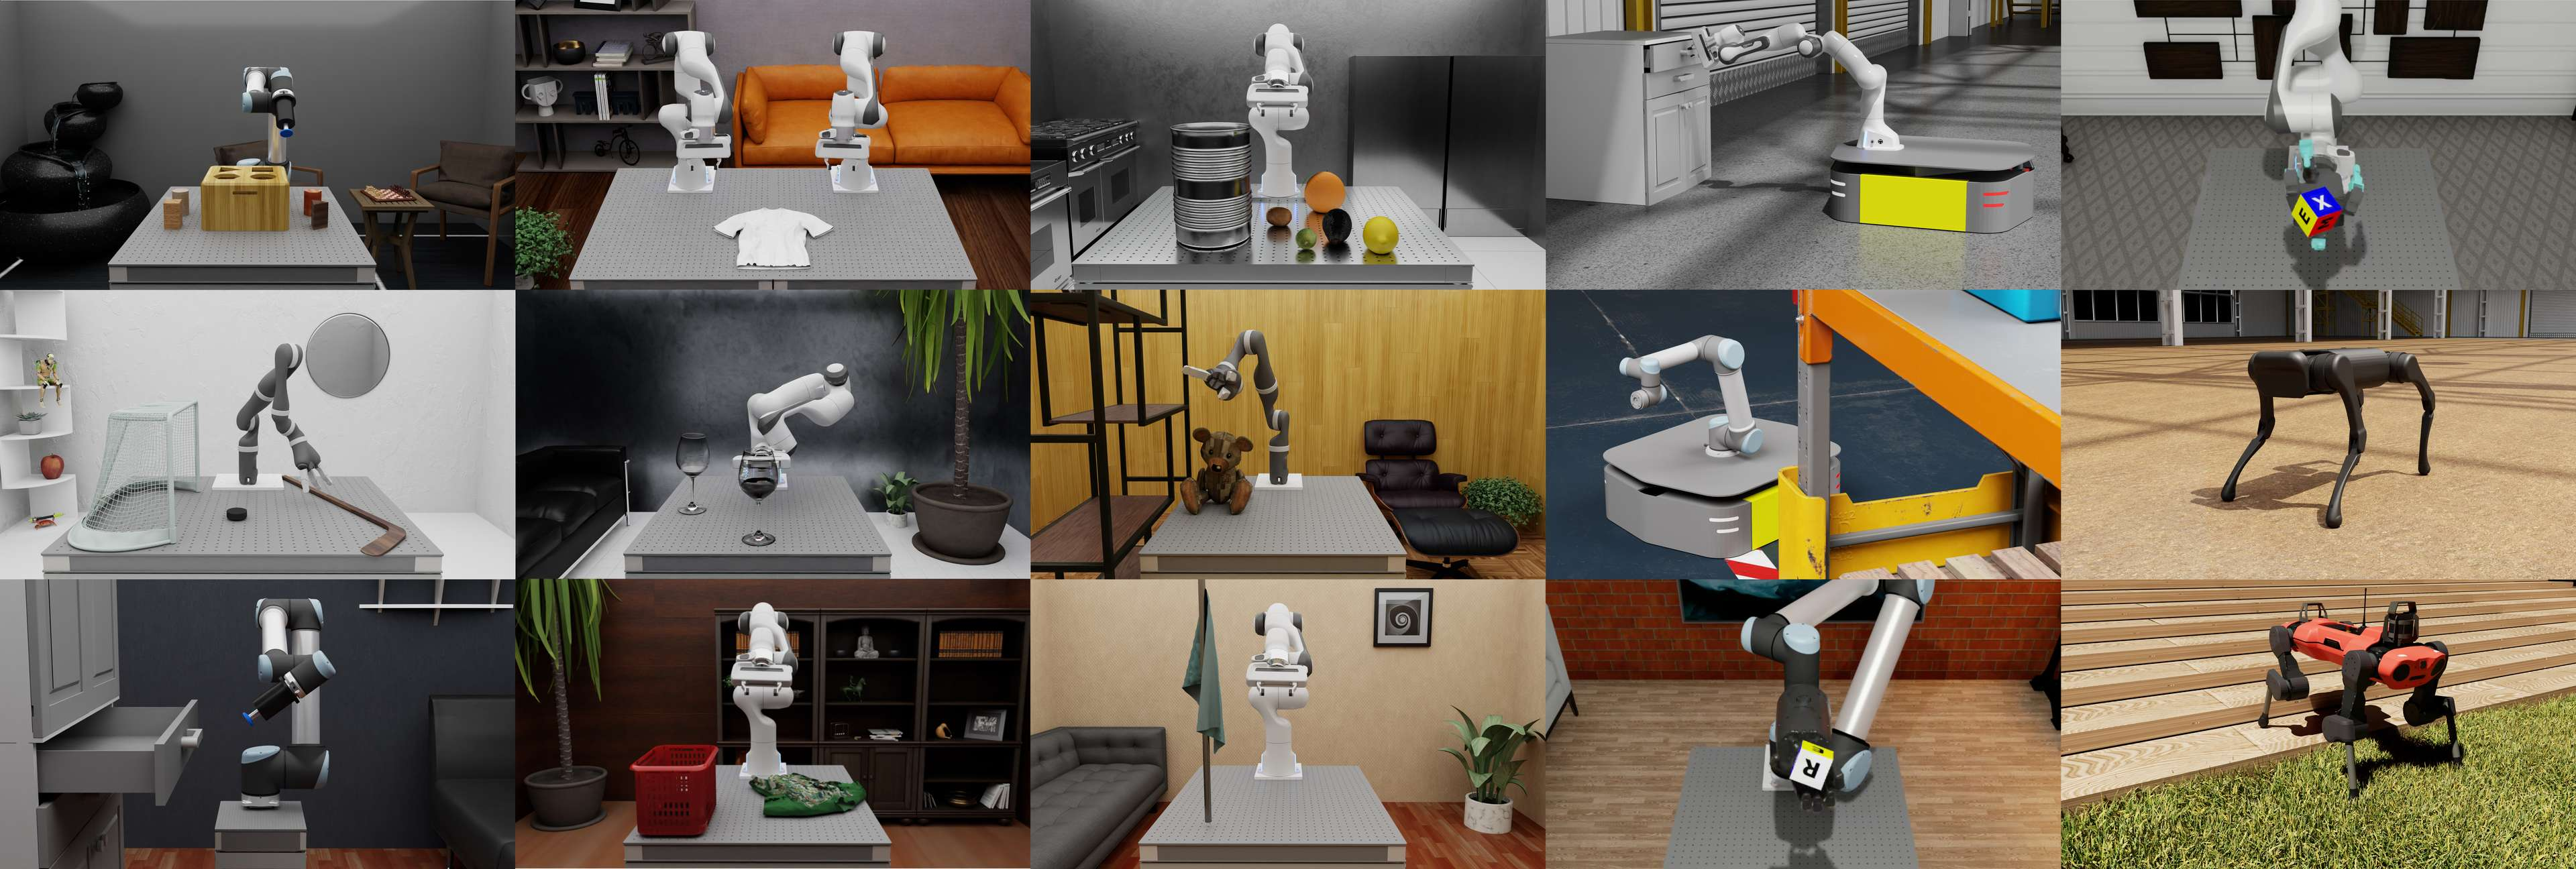
\includegraphics[width=0.85\textwidth]{figure/isaaclab_ecosystem.png}
    \caption{Kiến trúc cascade RL-PID hai tầng trong Isaac Lab}
    \label{fig:cascade_rl}
\end{figure}


% ==============================================
\subsection{Bước 1: Huấn luyện vòng trong (\texttt{Biped-Inner-Tilt})}
% ==============================================

\subsubsection{Thiết lập môi trường mô phỏng}

Môi trường được xây dựng trên Isaac Lab với lớp nền
\texttt{ManagerBasedRLEnvCfg}, sử dụng \textbf{512 môi trường song song}.
Mặt phẳng mô phỏng có hệ số ma sát tĩnh $\mu_s = 2{,}0$ và động
$\mu_k = 1{,}8$ — cao hơn so với điều kiện thực để đảm bảo bánh xe
không trượt trong giai đoạn học ban đầu.

Vòng lặp vật lý chạy ở \textbf{200~Hz}; chính sách vòng trong cũng
được gọi ở \textbf{200~Hz} (\texttt{decimation}~$= 1$) vì bộ điều
khiển PID cấp thấp cần tần số cao để phản ứng nhanh với sai lệch góc.
Mỗi episode kéo dài tối đa $T_{ep} = 15\;\text{s}$ (3\,000 bước).

\subsubsection{Không gian hành động}

Chính sách vòng trong xuất \textbf{21 hệ số PID thô}
$\mathbf{a}_{raw} \in [-1,1]^{21}$, được tổ chức thành 7 bộ
$\times$ 3 tham số $[k_p, k_i, k_d]$:

\begin{table}[H]
    \centering
    \caption{Cấu trúc hành động 21 chiều của vòng trong}
    \label{tab:inner_action}
    \renewcommand{\arraystretch}{1.3}
    \begin{tabular}{|c|l|l|}
    \hline
    \textbf{Chỉ số} & \textbf{Bộ điều khiển} & \textbf{Mục tiêu} \\
    \hline
    0 & PID vị trí hông \texttt{left\_hip\_joint\_A1}  & Góc khớp (rad) \\
    1 & PID vị trí hông \texttt{right\_hip\_joint\_A1} & Góc khớp (rad) \\
    2 & PID vị trí hông \texttt{left\_hip\_joint\_A2}  & Góc khớp (rad) \\
    3 & PID vị trí hông \texttt{right\_hip\_joint\_A2} & Góc khớp (rad) \\
    4 & PID cân bằng bánh xe trái (Segway)             & Sai lệch góc nghiêng (rad) \\
    5 & PID cân bằng bánh xe phải (Segway)             & Sai lệch góc nghiêng (rad) \\
    6 & PID yaw                                         & Sai lệch góc quay (rad) \\
    \hline
    \end{tabular}
\end{table}

\textbf{Ánh xạ hệ số thô → giá trị thực.}
Mỗi hành động thô $a_{raw} \in [-1, 1]$ được chuyển về miền giá trị
thực qua công thức tuyến tính:
\begin{equation}
    k = \operatorname{clamp}\!\bigl(a_{raw} \times \text{scale} \times s + b,\; 0,\; \infty\bigr)
    \label{eq:gain_mapping}
\end{equation}
với $s = (k_{max} - k_{min})/2$ và $b = (k_{max} + k_{min})/2$.
Kết quả được clamp về $[0, \infty)$ để đảm bảo hệ số PID không âm.
Bảng~\ref{tab:gain_bounds} liệt kê miền giá trị theo từng nhóm:

\begin{table}[H]
    \centering
    \caption{Miền giá trị hệ số PID theo nhóm}
    \label{tab:gain_bounds}
    \renewcommand{\arraystretch}{1.3}
    \begin{tabular}{|l|c|c|c|c|c|c|}
    \hline
    \textbf{Nhóm PID} & $k_{p,min}$ & $k_{p,max}$ & $k_{i,min}$ & $k_{i,max}$ & $k_{d,min}$ & $k_{d,max}$ \\
    \hline
    Hông (vị trí)    & 10  & 160  & 0   & 6    & 0   & 6    \\
    Bánh xe (cân bằng)& 20  & 200  & 0   & 10   & 2   & 40   \\
    Yaw              & 1   & 16   & 0   & 0{,}6 & 0  & 2    \\
    \hline
    \end{tabular}
\end{table}

\subsubsection{Cơ chế điều khiển trong \texttt{apply\_actions()}}

Tại mỗi bước vật lý, \texttt{TiltPIDAction} thực hiện ba bước tính toán
và áp dụng mô-men xoắn lên robot:

\paragraph{1. PID vị trí hông.}
Vị trí đích 4 khớp hông được tính từ lệnh góc nghiêng và vecto phân bổ:
\begin{equation}
    q_{des,hip} = q_{default} + \phi_{des} \cdot \mathbf{r}_{roll}
                  + \theta_{des} \cdot \mathbf{r}_{pitch}
    \label{eq:hip_des}
\end{equation}
với $\mathbf{r}_{roll} = [0{,}5,\;{-}0{,}5,\;0{,}5,\;{-}0{,}5]$ và
$\mathbf{r}_{pitch} = [0{,}3,\;0{,}3,\;0{,}3,\;0{,}3]$.
Mô-men hông:
\begin{equation}
    \tau_{hip} = \operatorname{clamp}\!\bigl(
        k_p (q_{des} - q) + k_i \int(q_{des}-q)\,dt + k_d(-\dot{q}),\;
        \pm 160\;\text{N·m}\bigr)
    \label{eq:hip_pid}
\end{equation}

\paragraph{2. PID cân bằng bánh xe (cơ chế Segway).}
Bánh xe bù sai lệch góc nghiêng theo cơ chế con lắc ngược trên bánh xe:
\begin{align}
    e_L &= e_{roll} + \alpha_{diff} \cdot e_{pitch}, \quad
    e_R = e_{roll} - \alpha_{diff} \cdot e_{pitch}
    \label{eq:wheel_err} \\
    \tau_{balance} &= -\operatorname{clamp}\!\bigl(
        k_p e + k_i \int e\,dt + k_d (-\dot{\phi}),\;
        \pm 120\;\text{N·m}\bigr)
    \label{eq:wheel_balance}
\end{align}
với $\alpha_{diff} = 0{,}5$ là hệ số phân bổ vi sai trái-phải.

\paragraph{3. PID yaw.}
\begin{equation}
    \tau_{yaw} = \operatorname{clamp}\!\bigl(
        k_p e_\psi + k_i \int e_\psi\,dt + k_d(-\dot{\psi}),\;
        \pm 20\;\text{N·m}\bigr)
    \label{eq:yaw_pid}
\end{equation}

\paragraph{4. Kết hợp mô-men bánh xe.}
\begin{equation}
    \tau_{wheel,L} = \tau_{balance,L} + \tau_{yaw}, \qquad
    \tau_{wheel,R} = \tau_{balance,R} - \tau_{yaw}
    \label{eq:wheel_combine}
\end{equation}

\subsubsection{Không gian quan sát}

Cả Actor lẫn Critic đều dùng chung một nhóm quan sát duy nhất
(\texttt{obs\_groups = \{"policy": ["policy"], "critic": ["policy"]\}}),
gồm \textbf{77 chiều}:

\begin{table}[H]
    \centering
    \caption{Không gian quan sát 77 chiều — task \texttt{Biped-Inner-Tilt}}
    \label{tab:obs_inner}
    \renewcommand{\arraystretch}{1.3}
    \begin{tabular}{|l|c|l|}
    \hline
    \textbf{Tín hiệu} & \textbf{Chiều} & \textbf{Mô tả} \\
    \hline
    \texttt{tilt\_error}       & 3  & $[\phi_{err}, \theta_{err}, \psi_{err}]$ — sai lệch roll/pitch/yaw (rad) \\
    \texttt{imu\_quat}         & 4  & Quaternion hướng thân $[q_w, q_x, q_y, q_z]$ \\
    \texttt{imu\_lin\_acc\_b}  & 3  & Gia tốc tuyến tính trong hệ thân $[a_x,a_y,a_z]$ (m/s$^2$) \\
    \texttt{ang\_vel\_b}       & 3  & Vận tốc góc trong hệ thân $[\omega_x, \omega_y, \omega_z]$ (rad/s) \\
    \texttt{projected\_gravity}& 3  & Vector trọng lực đơn vị chiếu vào hệ thân \\
    \texttt{hip\_pos\_error}   & 4  & $q_{des,hip} - q_{hip}$ (4 khớp hông) \\
    \texttt{hip\_vel}          & 4  & $\dot{q}_{hip}$ (4 khớp hông) (rad/s) \\
    \texttt{wheel\_vel}        & 2  & $[\omega_L, \omega_R]$ tốc độ góc bánh xe (rad/s) \\
    \texttt{all\_joint\_pos}   & 10 & Vị trí tất cả 10 khớp (tương đối so với mặc định) \\
    \texttt{all\_joint\_vel}   & 10 & Vận tốc tất cả 10 khớp (rad/s) \\
    \texttt{all\_joint\_acc}   & 10 & Gia tốc tất cả 10 khớp (rad/s$^2$) \\
    \texttt{last\_action}      & 21 & 21 hành động (hệ số PID) ở bước trước \\
    \hline
    \textbf{Tổng}              & \textbf{77} & \\
    \hline
    \end{tabular}
\end{table}

\subsubsection{Lệnh điều khiển}

Mỗi episode, Isaac Lab lấy mẫu ngẫu nhiên lệnh góc nghiêng mục tiêu
(\texttt{target\_tilt}) và duy trì trong $[5,\,10]\;\text{s}$ trước khi
resample. Lệnh mô phỏng tín hiệu bậc thang ngẫu nhiên — phù hợp để
đánh giá chất lượng đáp ứng bước nhảy:

\begin{table}[H]
    \centering
    \caption{Cấu hình lệnh góc nghiêng (\texttt{target\_tilt})}
    \label{tab:tilt_cmd}
    \renewcommand{\arraystretch}{1.3}
    \begin{tabular}{|l|c|l|}
    \hline
    \textbf{Thành phần} & \textbf{Miền giá trị} & \textbf{Ý nghĩa} \\
    \hline
    $\phi_{des}$ (roll)       & $[-0{,}05,\;+0{,}05]$ rad ($\approx\pm2{,}9°$)  & Góc nghiêng ngang \\
    $\theta_{des}$ (pitch)    & $[-0{,}05,\;+0{,}05]$ rad ($\approx\pm2{,}9°$)  & Góc nghiêng dọc \\
    $\Delta\psi$ (yaw delta)  & $[-0{,}30,\;+0{,}30]$ rad ($\approx\pm17{,}2°$) & Thay đổi góc quay \\
    Thời gian giữ             & $[5{,}0,\;10{,}0]$ s & Khoảng resample \\
    \hline
    \end{tabular}
\end{table}

\subsubsection{Sự kiện reset}

Tại mỗi lần khởi động lại episode, hai sự kiện reset được áp dụng:
\begin{itemize}
    \item \textbf{Reset vị trí thân} (\texttt{reset\_root\_state\_uniform}):
    vị trí $(x,y) \sim \mathcal{U}(-0{,}05,\,+0{,}05)\;\text{m}$,
    góc roll/pitch $\sim \mathcal{U}(-0{,}05,\,+0{,}05)$~rad ($\approx\pm2{,}9°$),
    yaw $\sim \mathcal{U}(-\pi,\,+\pi)$~rad.

    \item \textbf{Reset khớp} (\texttt{reset\_joints\_by\_offset}):
    $\Delta q \sim \mathcal{U}(-0{,}02,\,+0{,}02)$~rad,
    $\Delta\dot{q} \sim \mathcal{U}(-0{,}10,\,+0{,}10)$~rad/s.
\end{itemize}

\subsubsection{Hàm phần thưởng}

Hàm phần thưởng đánh giá chất lượng đáp ứng bước nhảy trên ba tiêu chí:
bám góc nghiêng, đặc tính bước nhảy và mượt mà tín hiệu.

\begin{table}[H]
    \centering
    \caption{Hàm phần thưởng — task \texttt{Biped-Inner-Tilt}}
    \label{tab:rewards_inner}
    \renewcommand{\arraystretch}{1.3}
    \begin{tabular}{|l|c|p{7cm}|}
    \hline
    \textbf{Tên} & \textbf{Trọng số $w$} & \textbf{Ý nghĩa} \\
    \hline
    \multicolumn{3}{|c|}{\textit{Bám góc nghiêng}} \\
    \hline
    \texttt{termination\_penalty} & $-200$            & Phạt khi episode kết thúc sớm \\
    \texttt{tilt\_tracking\_exp}  & $+10{,}0$         & Gaussian: roll/pitch error, $\sigma=0{,}05$ \\
    \texttt{yaw\_tracking\_exp}   & $+3{,}0$          & Gaussian: yaw error, $\sigma=0{,}1$ \\
    \texttt{tilt\_tracking\_l2}   & $-2{,}0$          & Phạt $L_2$: roll$^2$ + pitch$^2$ \\
    \hline
    \multicolumn{3}{|c|}{\textit{Chất lượng đáp ứng bước nhảy}} \\
    \hline
    \texttt{settling\_bonus}      & $+5{,}0$          & Bonus khi $|\phi_{err}|,|\theta_{err}|<0{,}03$ và $|\psi_{err}|<0{,}05$ \\
    \texttt{overshoot\_penalty}   & $-3{,}0$          & Phạt khi góc vượt qua setpoint (đổi dấu) \\
    \texttt{oscillation\_penalty} & $-2{,}0$          & Phạt tốc độ góc đảo chiều gần setpoint \\
    \hline
    \multicolumn{3}{|c|}{\textit{Mượt mà tín hiệu}} \\
    \hline
    \texttt{hip\_torque}   & $-1\times10^{-4}$ & $L_2$ mô-men 4 khớp hông \\
    \texttt{wheel\_torque} & $-1\times10^{-4}$ & $L_2$ mô-men 2 bánh xe \\
    \texttt{action\_rate}  & $-0{,}01$         & $L_2$ thay đổi hệ số PID giữa 2 bước \\
    \hline
    \end{tabular}
\end{table}

Các số hạng tracking dùng hàm mũ để có gradient khác 0 kể cả khi sai
số lớn:
\begin{align}
    r_{tilt} &= w_{tilt} \cdot \exp\!\left(-\frac{\phi_{err}^2 + \theta_{err}^2}{\sigma_{tilt}^2}\right),
    \quad \sigma_{tilt} = 0{,}05\;\text{rad}
    \label{eq:rew_tilt_exp} \\
    r_{yaw}  &= w_{yaw} \cdot \exp\!\left(-\frac{\psi_{err}^2}{\sigma_{yaw}^2}\right),
    \quad \sigma_{yaw} = 0{,}1\;\text{rad}
    \label{eq:rew_yaw_exp}
\end{align}
Tổng phần thưởng mỗi bước: $R_k = \sum_j r_j^{(k)}$.

\subsubsection{Điều kiện kết thúc episode}

Ba điều kiện đồng thời được kích hoạt trong suốt quá trình huấn luyện:
\begin{itemize}
    \item \textbf{Hết thời gian} (\texttt{time\_out}): $t \geq 15\;\text{s}$.
    \item \textbf{Nghiêng quá giới hạn} (\texttt{bad\_orientation}):
    góc nghiêng $> \pi/4{,}5 \approx 40°$ so với phương đứng.
    \item \textbf{Robot ngã xuống} (\texttt{fallen}):
    chiều cao thân $< 0{,}10\;\text{m}$.
\end{itemize}
Khi kết thúc sớm bởi hai điều kiện sau, agent nhận phần thưởng phạt
$r_{term} = -200$.


% ==============================================
\subsection{Bước 2: Huấn luyện vòng ngoài (\texttt{Biped-Outer-Angle})}
% ==============================================

\subsubsection{Nguyên tắc cascade}

Sau khi vòng trong được huấn luyện xong, trọng số mạng được đóng băng
và nhúng vào \texttt{BalanceCascadeActionCfg}. Vòng ngoài chỉ xuất
\textbf{3 hệ số PID cân bằng ngoài}
$[k_{p\theta}, k_{i\theta}, k_{d\theta}]$ để tính vận tốc góc mong muốn
$\omega_{des}$ từ góc nghiêng; chính sách vòng trong (đóng băng) nhận
$\omega_{des}$ làm setpoint và điều khiển mô-men xoắn ở 200~Hz bên trong
\texttt{apply\_actions()}.

\subsubsection{Thiết lập môi trường}

Môi trường vòng ngoài dùng \textbf{256 môi trường song song}, ma sát
$\mu_s = 0{,}85$, $\mu_k = 0{,}65$ (gần thực tế hơn). Chính sách ngoài
chạy ở \textbf{50~Hz} (\texttt{decimation}~$= 4$); episode tối đa
$T_{ep} = 20\;\text{s}$.

Reset ban đầu với tilt ngẫu nhiên $\pm 0{,}15\;\text{rad}$ ($\approx\pm8{,}6°$)
để tạo tín hiệu bậc thang cho vòng ngoài học đáp ứng.

\subsubsection{Không gian quan sát và hành động}

\begin{table}[H]
    \centering
    \caption{Quan sát 11 chiều — task \texttt{Biped-Outer-Angle}}
    \label{tab:obs_outer}
    \renewcommand{\arraystretch}{1.3}
    \begin{tabular}{|l|c|l|}
    \hline
    \textbf{Tín hiệu} & \textbf{Chiều} & \textbf{Mô tả} \\
    \hline
    \texttt{projected\_gravity} & 3 & Vector trọng lực chiếu trong hệ thân \\
    \texttt{ang\_vel\_b}        & 3 & Vận tốc góc thân $[\omega_x,\omega_y,\omega_z]$ (rad/s) \\
    \texttt{wheel\_vel}         & 2 & $[\omega_L, \omega_R]$ (rad/s) \\
    \texttt{last\_action}       & 3 & 3 hệ số PID ngoài bước trước \\
    \hline
    \textbf{Tổng}               & \textbf{11} & \\
    \hline
    \end{tabular}
\end{table}

Hành động 3 chiều $[k_{p\theta}, k_{i\theta}, k_{d\theta}]$ tương tự ánh xạ
\eqref{eq:gain_mapping}. Vòng ngoài không có lệnh tốc độ — mục tiêu duy nhất
là giữ robot thẳng đứng ($\phi = \theta = 0$).

\subsubsection{Hàm phần thưởng và điều kiện kết thúc}

\begin{table}[H]
    \centering
    \caption{Hàm phần thưởng — task \texttt{Biped-Outer-Angle}}
    \label{tab:rewards_outer}
    \renewcommand{\arraystretch}{1.3}
    \begin{tabular}{|l|c|p{7cm}|}
    \hline
    \textbf{Tên} & \textbf{Trọng số $w$} & \textbf{Ý nghĩa} \\
    \hline
    \texttt{termination\_penalty} & $-500$            & Phạt khi ngã (nặng hơn vòng trong) \\
    \texttt{balance\_exp}         & $+10{,}0$         & Gaussian cân bằng, $\sigma=0{,}1$ \\
    \texttt{balance\_l2}          & $-2{,}0$          & Phạt $L_2$ góc nghiêng \\
    \texttt{settling\_bonus}      & $+3{,}0$          & Bonus khi nghiêng $< 0{,}03\;\text{rad}$ \\
    \texttt{overshoot\_penalty}   & $-5{,}0$          & Phạt vượt điểm cân bằng \\
    \texttt{oscillation\_penalty} & $-2{,}0$          & Phạt dao động gần thẳng đứng \\
    \texttt{wheel\_vel\_l2}       & $-1\times10^{-3}$ & Phạt tốc độ bánh xe $L_2$ \\
    \texttt{torque\_l2}           & $-1\times10^{-5}$ & Phạt tổng mô-men xoắn $L_2$ \\
    \texttt{action\_rate}         & $-0{,}01$         & $L_2$ thay đổi hệ số PID ngoài \\
    \hline
    \end{tabular}
\end{table}

Điều kiện kết thúc tương tự vòng trong: \texttt{time\_out} ($t\geq20\;\text{s}$),
\texttt{bad\_orientation} ($> \pi/5 = 36°$) và \texttt{fallen} ($z < 0{,}10\;\text{m}$).


% ==============================================
\subsection{Thuật toán PPO và cấu trúc mạng}
% ==============================================

\subsubsection{Kiến trúc mạng}

Cả Actor và Critic dùng chung kiến trúc MLP 2 lớp ẩn với hàm kích hoạt
ELU, chuẩn hóa quan sát bằng running mean/std:

\begin{table}[H]
    \centering
    \caption{Kiến trúc mạng Actor-Critic}
    \label{tab:network_arch}
    \renewcommand{\arraystretch}{1.3}
    \begin{tabular}{|l|c|c|c|c|}
    \hline
    \textbf{Task} & \textbf{Đầu vào} & \textbf{Lớp ẩn} & \textbf{Đầu ra} & \textbf{Kích hoạt} \\
    \hline
    \texttt{Biped-Inner-Tilt}  & 77 & $[128 \to 128]$ & 21 (tuyến tính) & ELU \\
    \texttt{Biped-Outer-Angle} & 11 & $[128 \to 128]$ & 3  (tuyến tính) & ELU \\
    \hline
    \end{tabular}
\end{table}

Actor xuất phân phối Gaussian với $\boldsymbol{\mu}_a$ từ mạng và
$\sigma_{noise} = 0{,}1$ ban đầu.

\subsubsection{Cấu hình thuật toán PPO}

Thuật toán PPO~\cite{schulman2017ppo} được triển khai qua thư viện
\texttt{rsl\_rl}:

\begin{table}[H]
    \centering
    \caption{Siêu tham số PPO}
    \label{tab:ppo_cfg}
    \renewcommand{\arraystretch}{1.3}
    \begin{tabular}{|l|c|l|}
    \hline
    \textbf{Tham số} & \textbf{Giá trị} & \textbf{Ý nghĩa} \\
    \hline
    \multicolumn{3}{|c|}{\textit{Rollout \& Huấn luyện}} \\
    \hline
    \texttt{num\_steps\_per\_env}  & 48      & Số bước rollout mỗi môi trường / iteration \\
    \texttt{max\_iterations}       & 5\,000  & Tổng số iteration huấn luyện \\
    \texttt{num\_learning\_epochs} & 5       & Số epoch cập nhật mạng mỗi iteration \\
    \texttt{num\_mini\_batches}    & 4       & Số mini-batch mỗi epoch \\
    \hline
    \multicolumn{3}{|c|}{\textit{PPO Clip \& Loss}} \\
    \hline
    \texttt{clip\_param}           & 0{,}2   & Tham số clip $\epsilon$ \\
    \texttt{value\_loss\_coef}     & 1{,}0   & Hệ số loss hàm giá trị $c_1$ \\
    \texttt{entropy\_coef}         & 0{,}01  & Hệ số entropy bonus $c_2$ \\
    \texttt{use\_clipped\_value\_loss} & True & Có clip value loss \\
    \hline
    \multicolumn{3}{|c|}{\textit{Optimizer \& Gradient}} \\
    \hline
    \texttt{learning\_rate}        & $3\times10^{-4}$ & Tốc độ học Adam \\
    \texttt{schedule}              & adaptive         & Điều chỉnh lr theo KL divergence \\
    \texttt{desired\_kl}           & 0{,}01           & Ngưỡng KL mục tiêu \\
    \texttt{max\_grad\_norm}       & 1{,}0            & Clipping gradient \\
    \hline
    \multicolumn{3}{|c|}{\textit{Ước tính lợi thế (GAE)}} \\
    \hline
    $\gamma$ (\texttt{gamma})      & 0{,}99  & Hệ số chiết khấu \\
    $\lambda$ (\texttt{lam})       & 0{,}95  & Tham số GAE \\
    \hline
    \end{tabular}
\end{table}

Tổng kích thước rollout buffer mỗi iteration với 512 môi trường (vòng trong):
\begin{equation}
    N_{buffer} = N_{envs} \times N_{steps} = 512 \times 48 = 24\,576\;\text{mẫu}
    \label{eq:buffer_size}
\end{equation}

Lợi thế được tính theo GAE:
\begin{equation}
    \hat{A}_t = \sum_{l=0}^{N-1} (\gamma\lambda)^l \delta_{t+l},
    \quad \delta_t = r_t + \gamma V(s_{t+1}) - V(s_t)
    \label{eq:gae}
\end{equation}

Hàm loss PPO:
\begin{equation}
    \mathcal{L}_{PPO} =
    -\underbrace{\mathbb{E}\!\left[\min\!\left(
        \rho_t \hat{A}_t,\;
        \operatorname{clip}(\rho_t, 1{\pm}\epsilon)\hat{A}_t
    \right)\right]}_{\mathcal{L}_{policy}}
    + c_1\,\underbrace{\mathbb{E}\!\left[(V_\theta(s_t) - V_t^{targ})^2\right]}_{\mathcal{L}_{value}}
    - c_2\,\underbrace{\mathbb{E}\!\left[H[\pi_\theta(\cdot|s_t)]\right]}_{\mathcal{L}_{entropy}}
    \label{eq:ppo_loss}
\end{equation}
với $\rho_t = \pi_\theta(a_t|s_t)/\pi_{\theta_{old}}(a_t|s_t)$,
$\epsilon = 0{,}2$, $c_1 = 1{,}0$, $c_2 = 0{,}01$.


% ==============================================
\subsection{Cấu hình phần cứng huấn luyện}
% ==============================================

\begin{table}[H]
    \centering
    \caption{Thông số GPU huấn luyện --- NVIDIA RTX 3070}
    \label{tab:gpu_spec}
    \renewcommand{\arraystretch}{1.3}
    \begin{tabular}{|l|l|}
    \hline
    \textbf{Thông số} & \textbf{Giá trị} \\
    \hline
    Kiến trúc         & NVIDIA Ampere \\
    CUDA Cores        & 5\,888 \\
    Tensor Cores      & 184 (thế hệ 3) \\
    VRAM              & 8\,GB GDDR6 \\
    Băng thông bộ nhớ & 448\,GB/s \\
    Hiệu năng FP32    & 20{,}3 TFLOPS \\
    \hline
    \end{tabular}
\end{table}

Ước tính bộ nhớ GPU khi huấn luyện vòng trong (512 env):
\begin{itemize}
    \item \textbf{Isaac Sim runtime} (PhysX): $\approx 1$--$2$\,GB.
    \item \textbf{Rollout buffer}: $512 \times 48 \times (77 + 21 + 3) \times 4\;\text{byte}
          \approx 19\;\text{MB}$.
    \item \textbf{Tham số mạng + optimizer}: $\approx 5\;\text{MB}$.
\end{itemize}
Tổng ước tính dưới $3\;\text{GB}$, phù hợp với 8\,GB VRAM của RTX 3070.
